\subsection{Experimentación sobre Kmeans}
\paragraph{}
Para los experimentos utilizamos las instancias de tipo A dadas por la cátedra. Los ejemplos de malos casos y problemas que puede llegar a tener kmeans fueron incluidos. Por ejemplo, los malos casos que acabamos de mencionar y sus diferentes tipos de entrada.
\paragraph{}
Para esta heurística y su experimentación tuvimos en cuenta principalmente dos cosas: el tamaño de la entrada y la forma en la que entran los datos o más directamente, como se recorren los puntos. Como vimos al analizar los casos, Kmeans depende de que centroids elige primero cuando la demanda es ajustada (recordemos la analogía de tetris que usamos). Por esto mismo, al experimentar sobre esta heurística decidimos tener en cuenta la forma en que se recorren los puntos (y en consecuencia, quienes tienen prioridad para asignarse a un cluster primero).
\paragraph{}
Una primera idea es ordenar los puntos por demanda, de manera decreciente. De esta forma, evitamos los casos en los que los camiones se van llenando de manera que quede bastante espacio en cada uno pero no el suficiente para albergar el producto de clientes de gran demanda. En casos en que esto no se tiene en cuenta, incluso podrían crearse nuevos clusters con centroid en esos clientes con alta demanda: lo cual puede significar en una mejora o no, dependiendo el caso. Por esto mismo, también decidimos experimentar con el caso contrario: en el que se de prioridad a los clientes con baja demanda, ordenando y recorriendo los puntos de manera creciente.
\paragraph{} 
Además de la experimentación mencionada, también chequeamos que la complejidad teórica que propusimos sea correcta o aproximada a la complejidad práctica del algoritmo.
\subsubsection{Sorting}

\begin{figure}[H]
	\centering
	\begin{minipage}{0.44\textwidth}
		\centering
		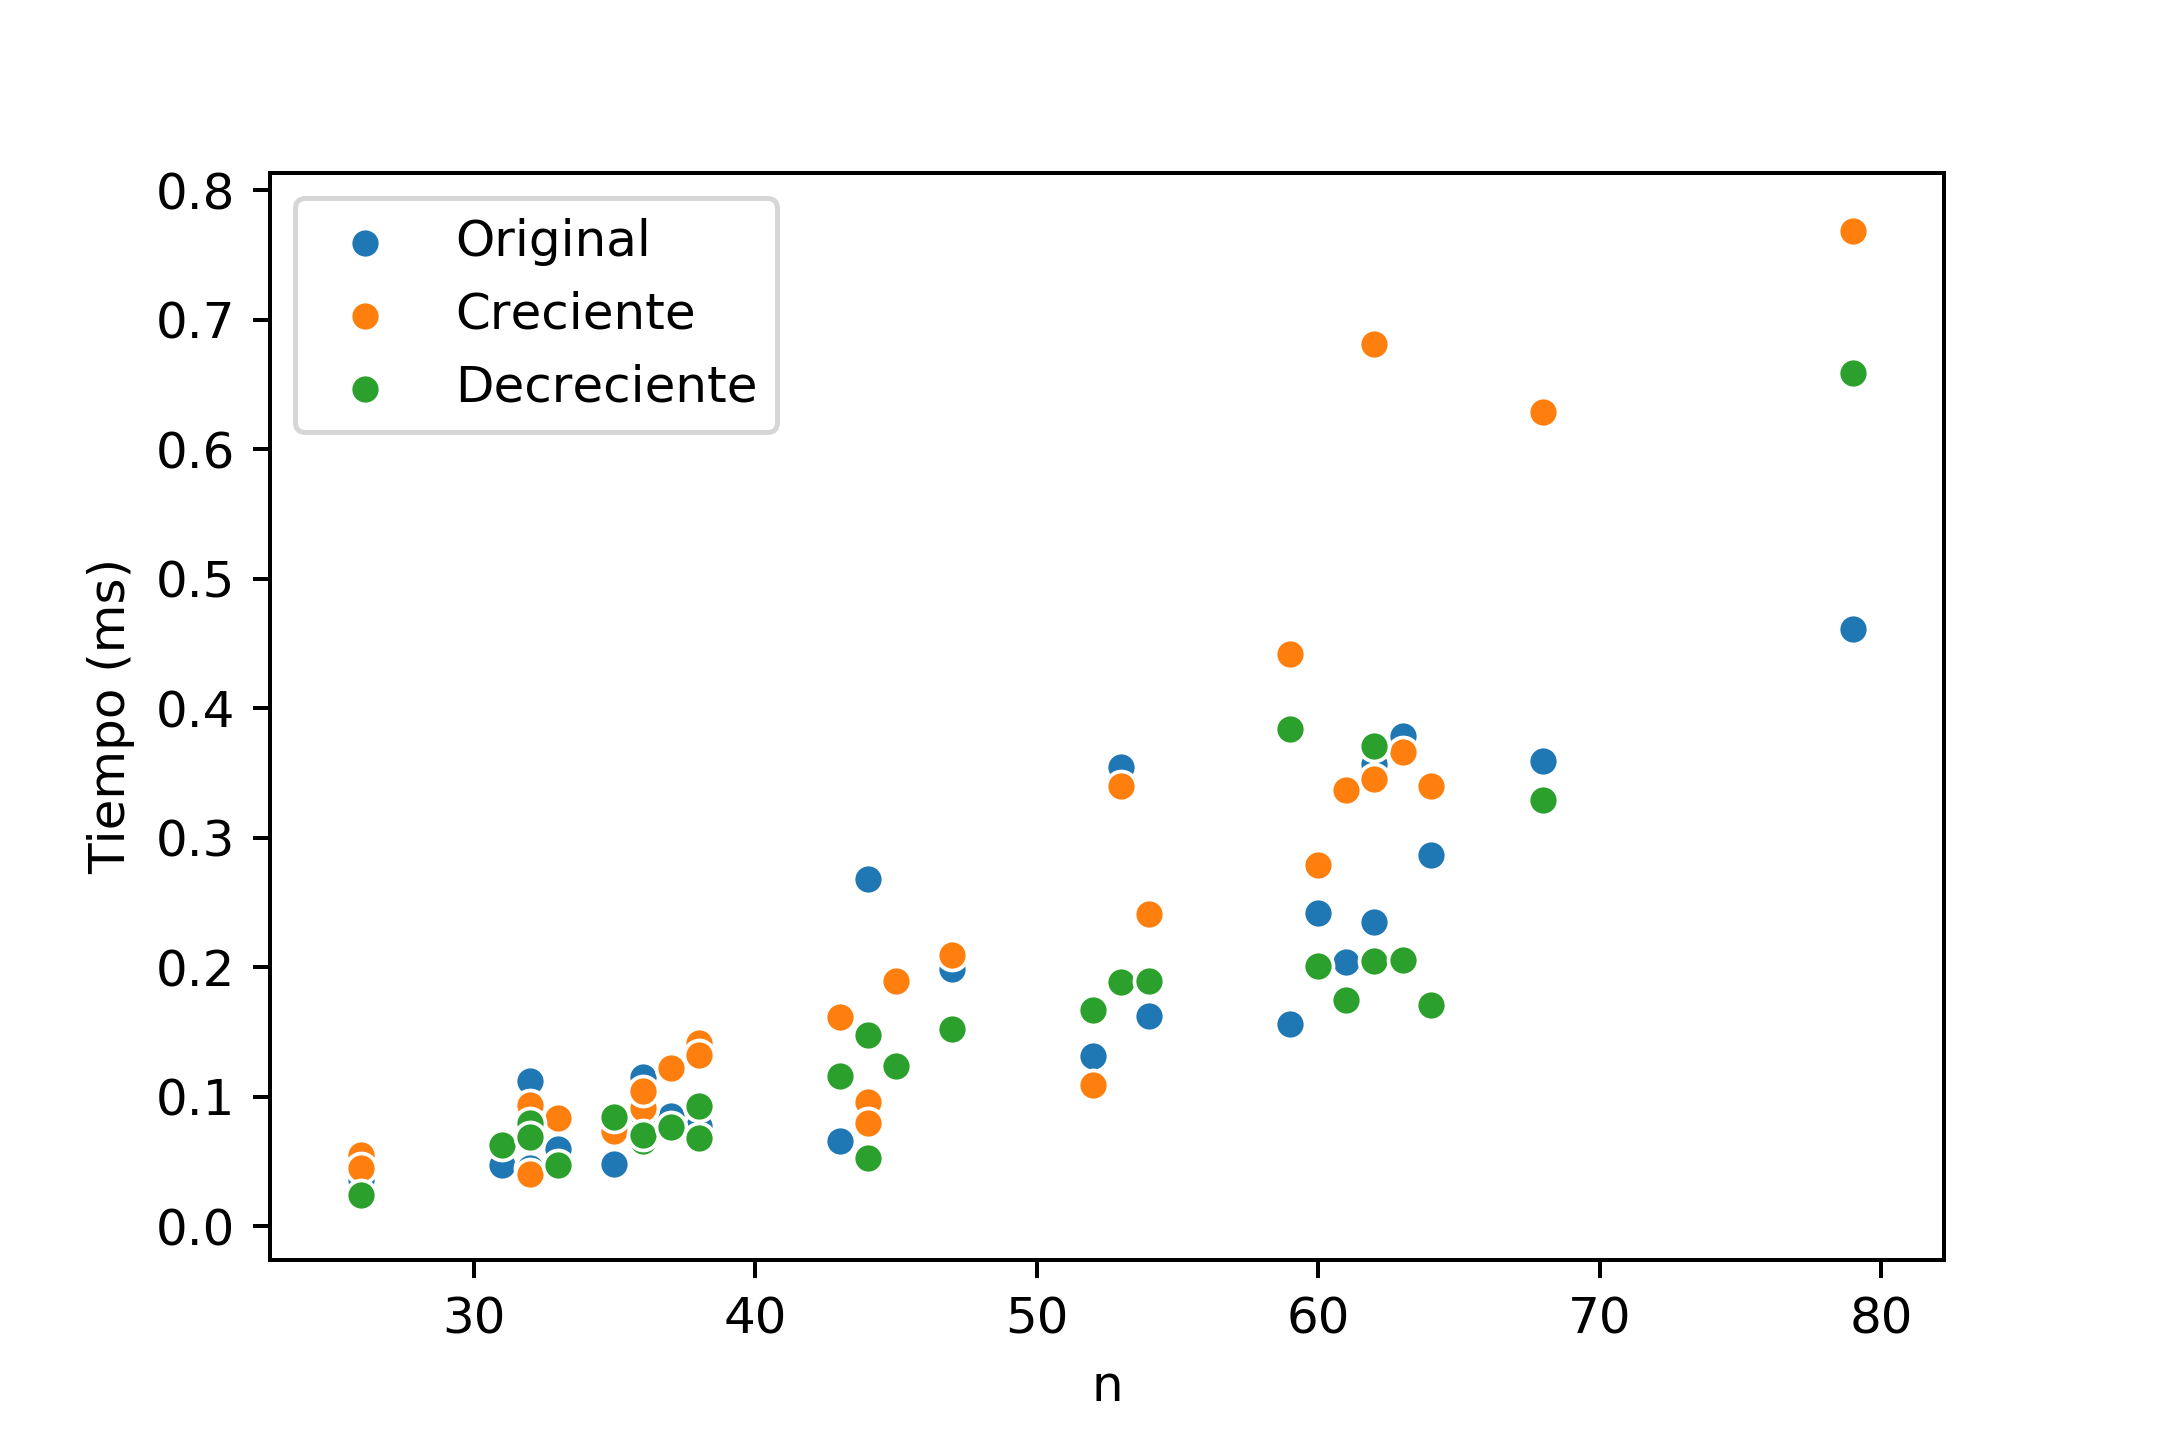
\includegraphics[width=1\textwidth]{images/kmeans/expsortingtiempo}
		\caption{\footnotesize Tiempo de acuerdo al tamaño de la entrada}
		\label{fig:kmeans-sort-tiempo}
	\end{minipage}%
	\hspace{0.03\textwidth}
	\begin{minipage}{0.44\textwidth}
		\centering
		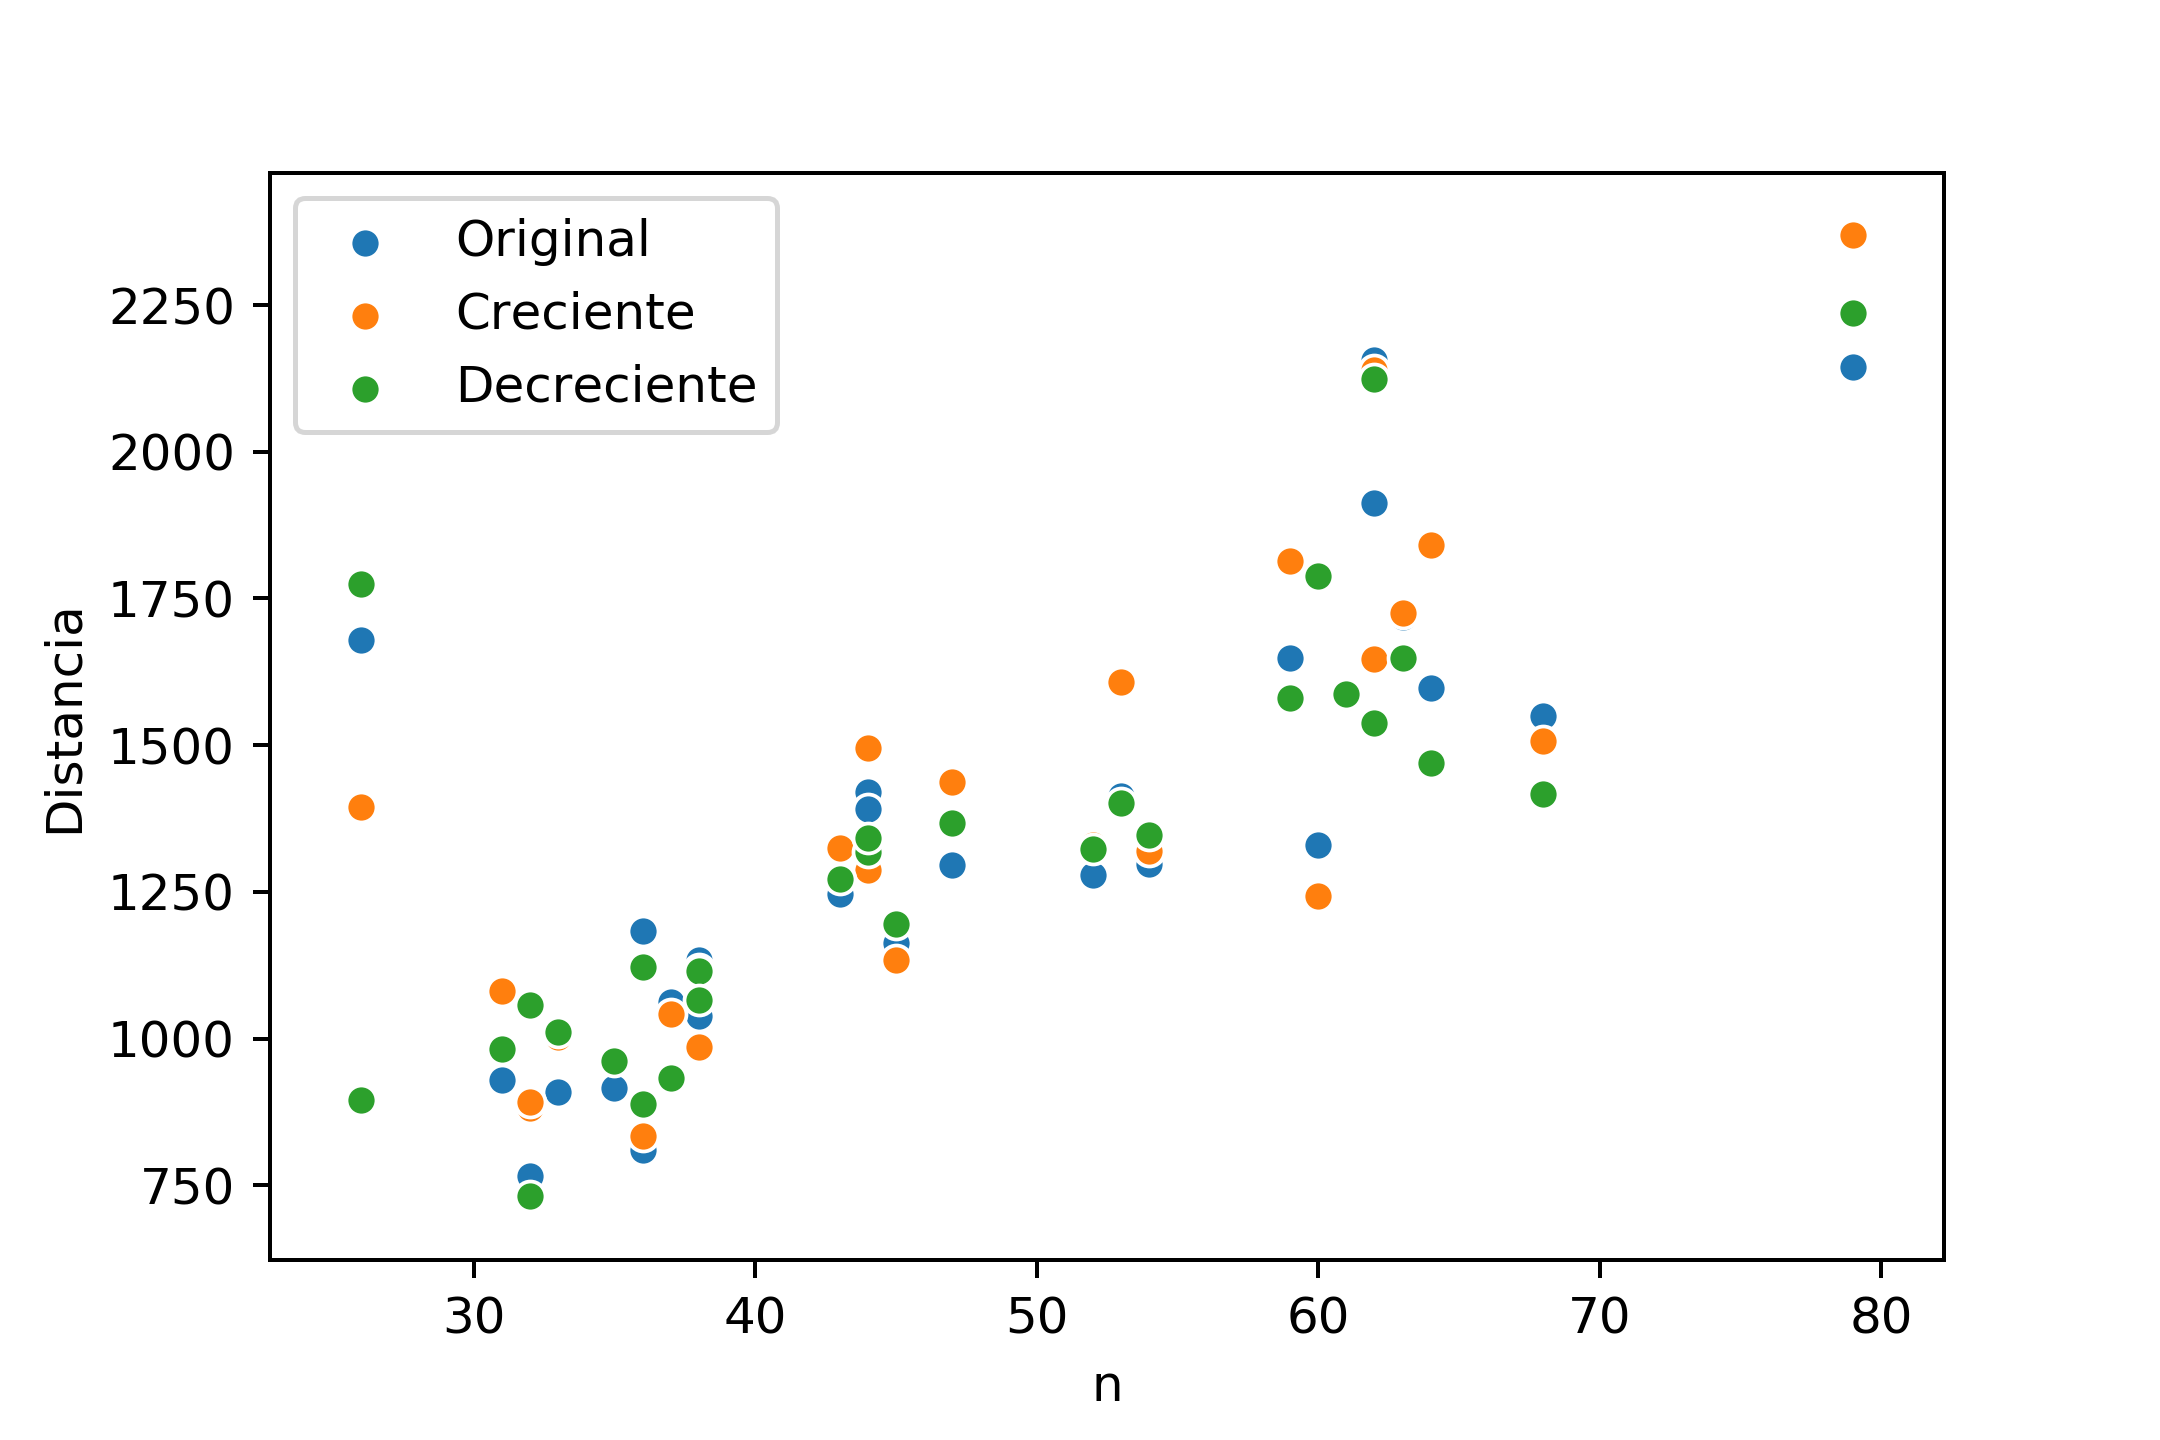
\includegraphics[width=1\textwidth]{images/kmeans/expsorting}
		\caption{\footnotesize Distancia de las soluciones obtenida de acuerdo al tamaño de la entrada}
		\label{fig:kmeans-sort-distancia}
	\end{minipage}%
\end{figure}

\begin{figure}[H]
	\centering
	\begin{minipage}{0.44\textwidth}
		\centering
		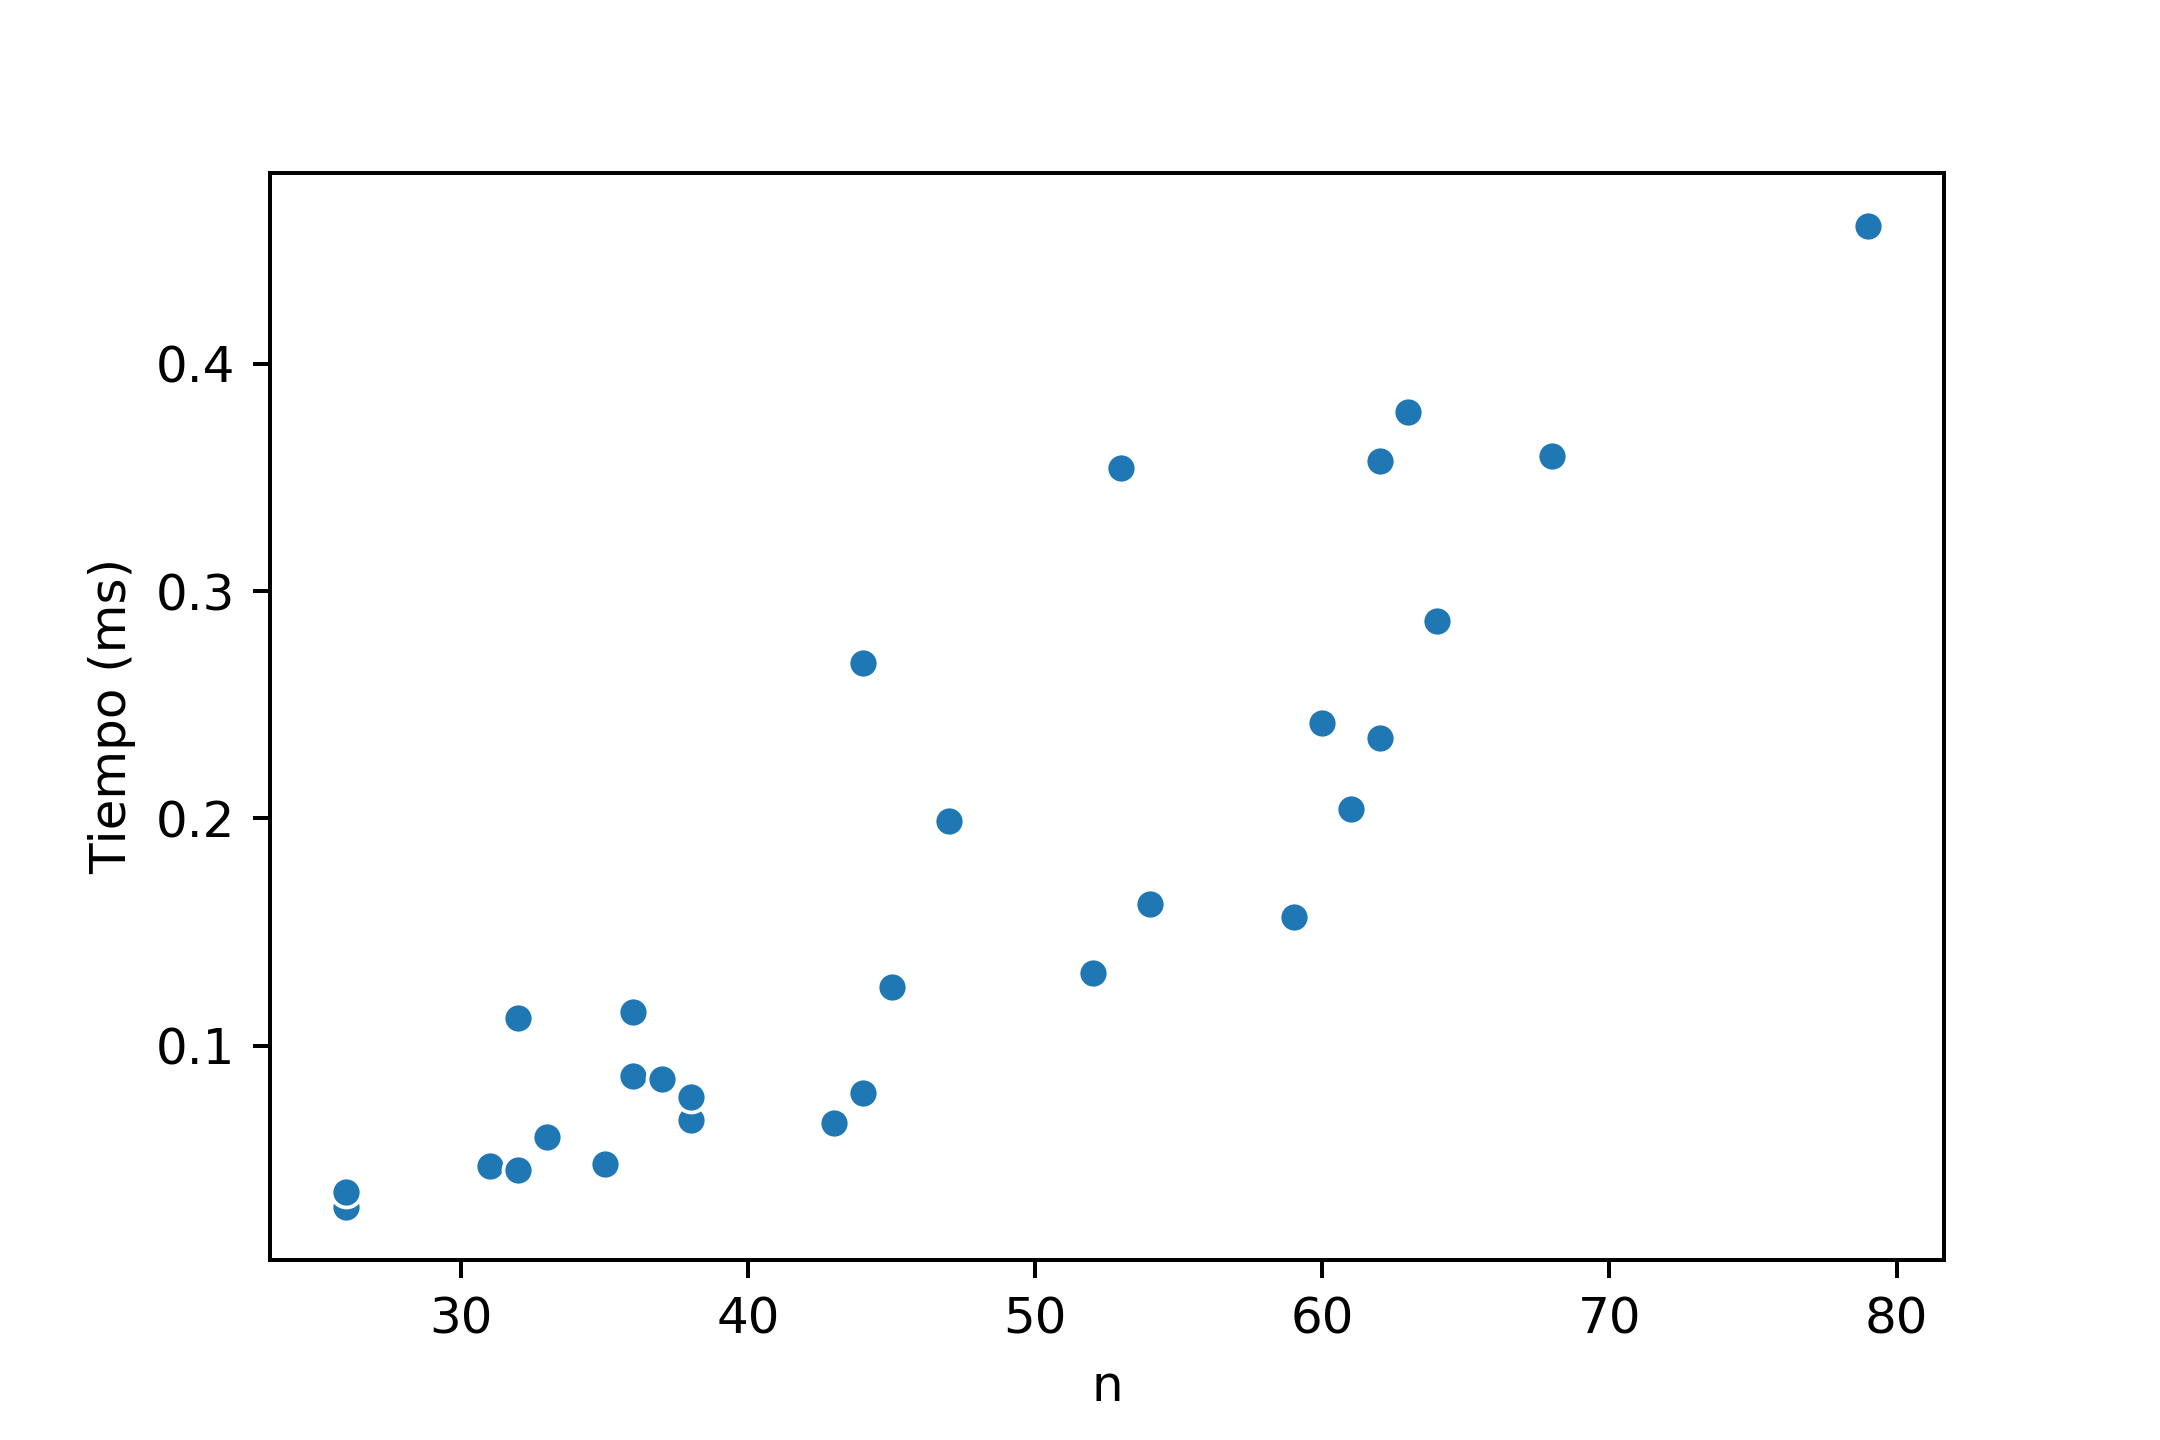
\includegraphics[width=1\textwidth]{images/kmeans/tiempokmeans}
		\caption{\footnotesize Tiempo de acuerdo al tamaño de la entrada}
		\label{fig:kmeans-tiempos}
	\end{minipage}%
	\hspace{0.03\textwidth}
	\begin{minipage}{0.44\textwidth}
		\centering
		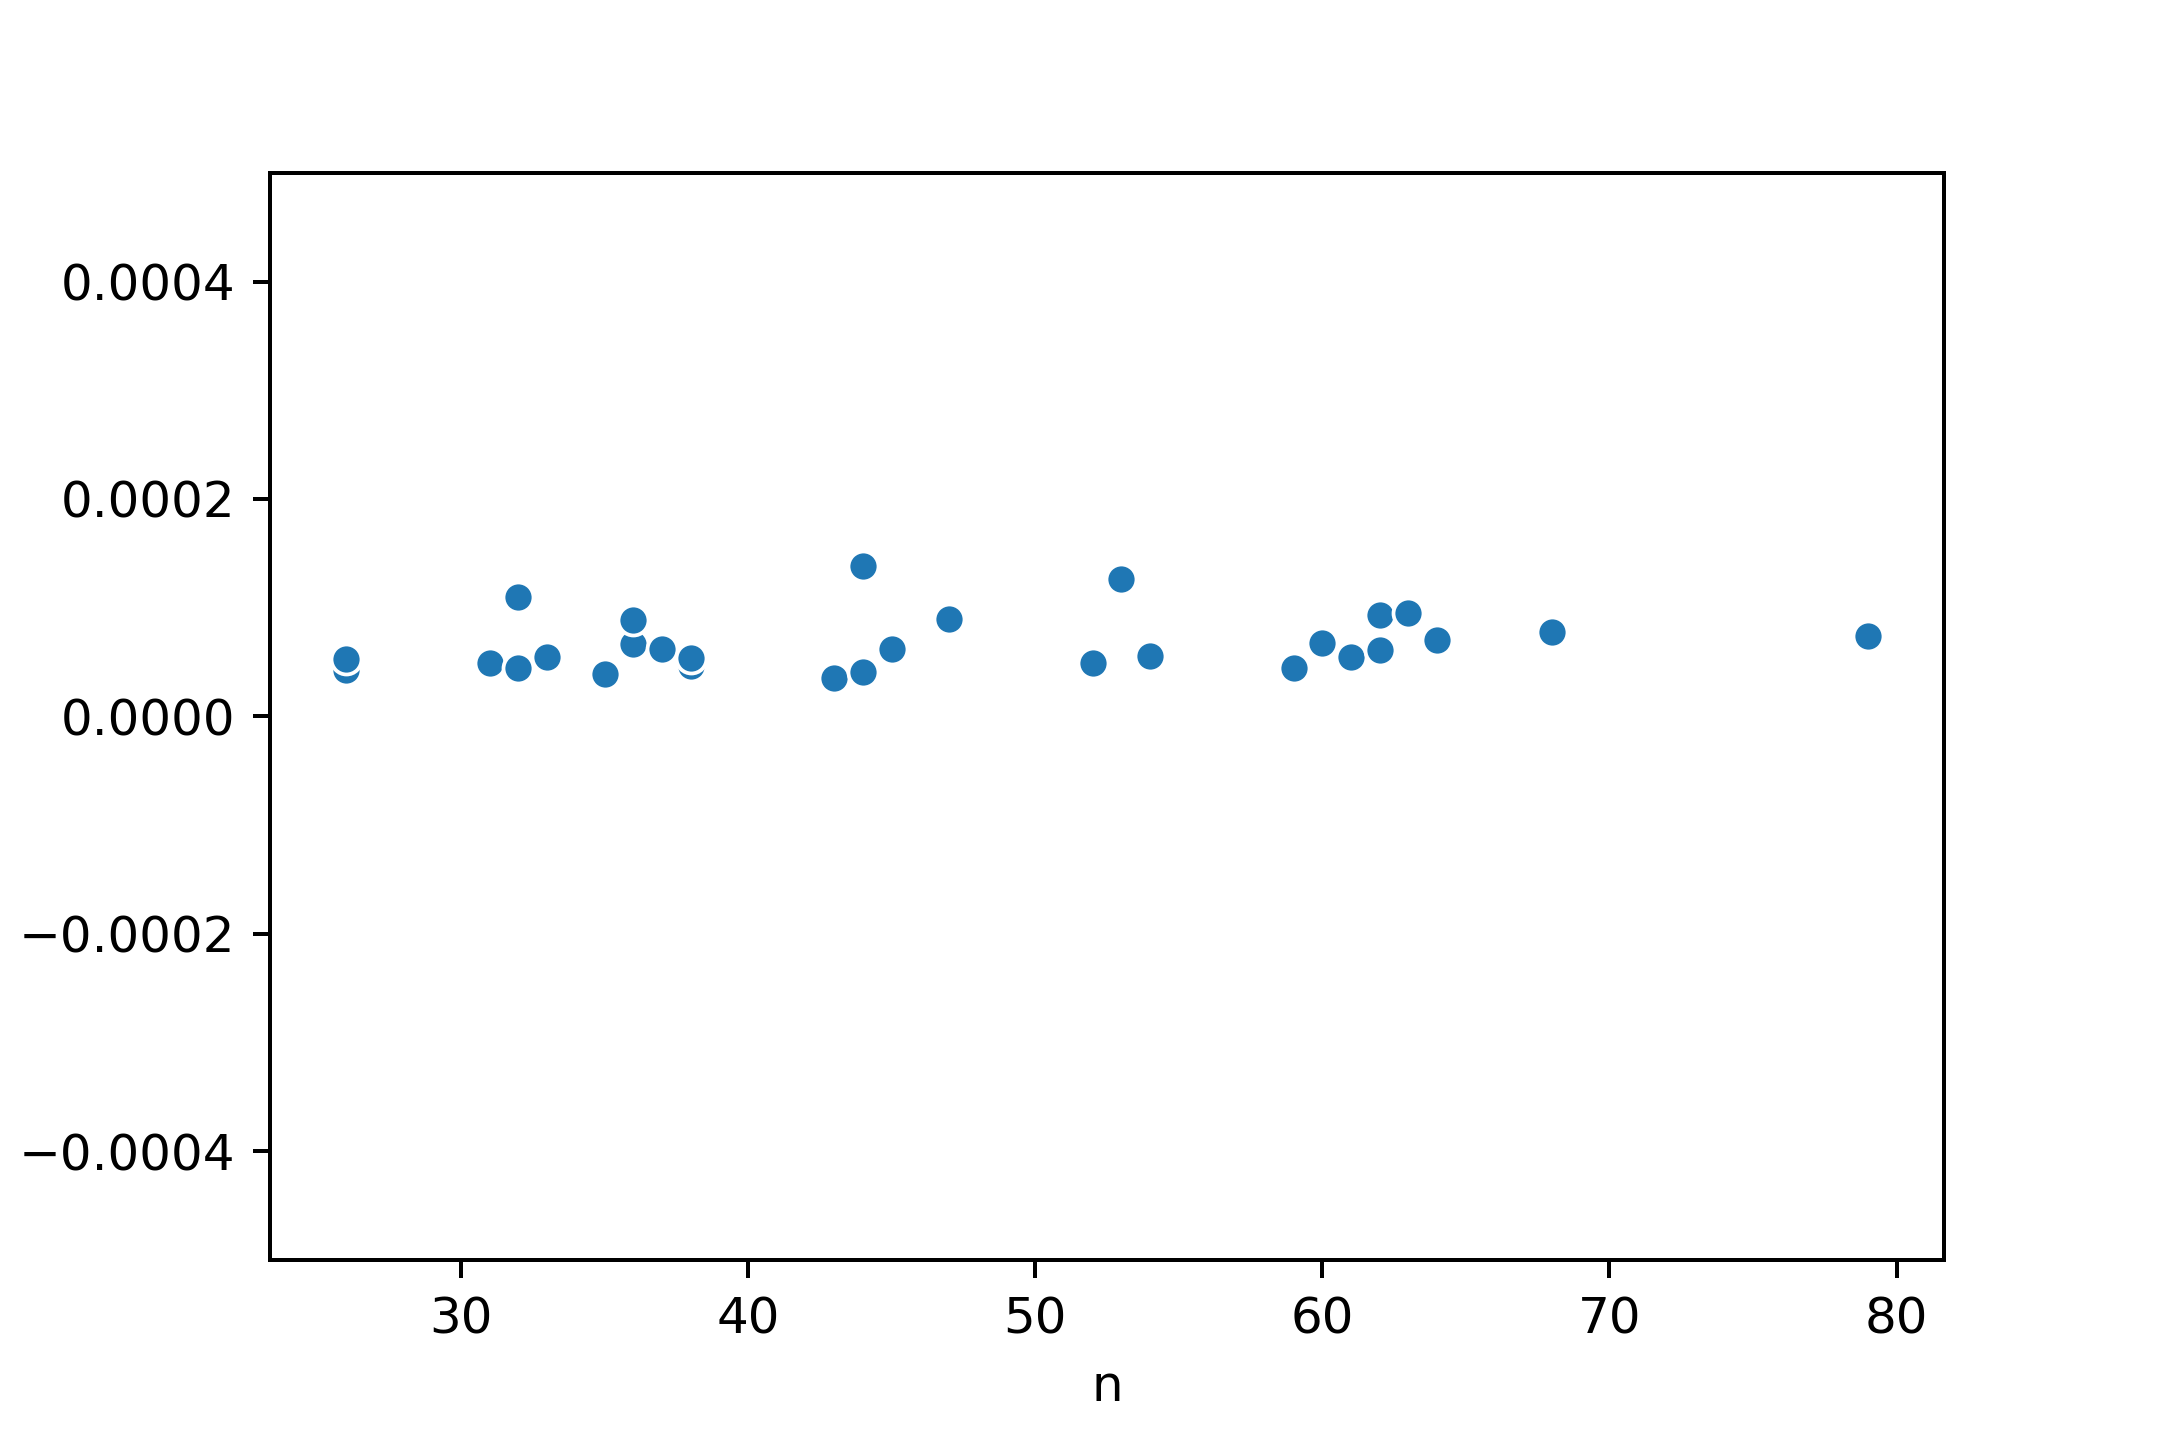
\includegraphics[width=1\textwidth]{images/kmeans/kmeanscte}
		\caption{\footnotesize Tiempo/complejidad de acuerdo al tamaño de la entrada}
		\label{fig:kmeans-cte}
	\end{minipage}%
\end{figure}

